\documentclass[11pt]{article}
\pdfpxdimen=1in
\divide\pdfpxdimen by 300
 
\usepackage[latin1]{inputenc}
\usepackage[T1]{fontenc}
\usepackage[english]{babel}
\usepackage{mathtools, bm}
\usepackage{amssymb, bm}
\usepackage{float}

\usepackage{caption} % to center captions
\usepackage{subcaption} % subcaption for figures side by side

\usepackage{booktabs} % for super cool table
\usepackage[table,xcdraw]{xcolor}  % to put color in tables
\usepackage{tcolorbox} % add box
\usepackage{commath} % for absolute values

\usepackage[parfill]{parskip}
\usepackage{graphicx}
\usepackage{hyperref}
\usepackage[top=0.8in, bottom=0.8in, left=1in, right=1in]{geometry}
\usepackage{listings}


\renewcommand\thesubsection{\thesection.\arabic{subsection}} % Subsection starting with A, B, ...

\renewcommand\thefigure{\thesubsection.\arabic{figure}}

\newcommand{\horrule}[1]{\rule{\linewidth}{#1}} % Create horizontal rule command with 1 argument of height

\numberwithin{figure}{section} % to have per-section figure numbering

\title{	
\normalfont \normalsize 
\textsc{Master MVA \\
Reinforcement Learning} \\ [20pt]
\horrule{0.5pt} \\[0.2cm] % Thin top horizontal rule
\textbf{TP 1}: Dynamic Programming and Reinforcement Learning \\
\horrule{2pt} \\[0.3cm] % Thick bottom horizontal rule
}

\author{Victor Busa \\
   \texttt{victor.busa@ens-paris-saclay.fr}}

\date{\normalsize\today}

\begin{document}

\maketitle

\section{Dynamic Programming}
\paragraph{Q1} See code
\paragraph{Q2} See code
\paragraph{Q3} For Policy Iteration, I used the Bellman operator $\mathcal{T}$ to evaluate the optimal policy. The Figure ~\ref{fig:error_rate} depicts the error rates for both Value Iteration and Policy Iteration.

\begin{figure}[H]
\centering
\begin{subfigure}{.5\textwidth}
  \centering
  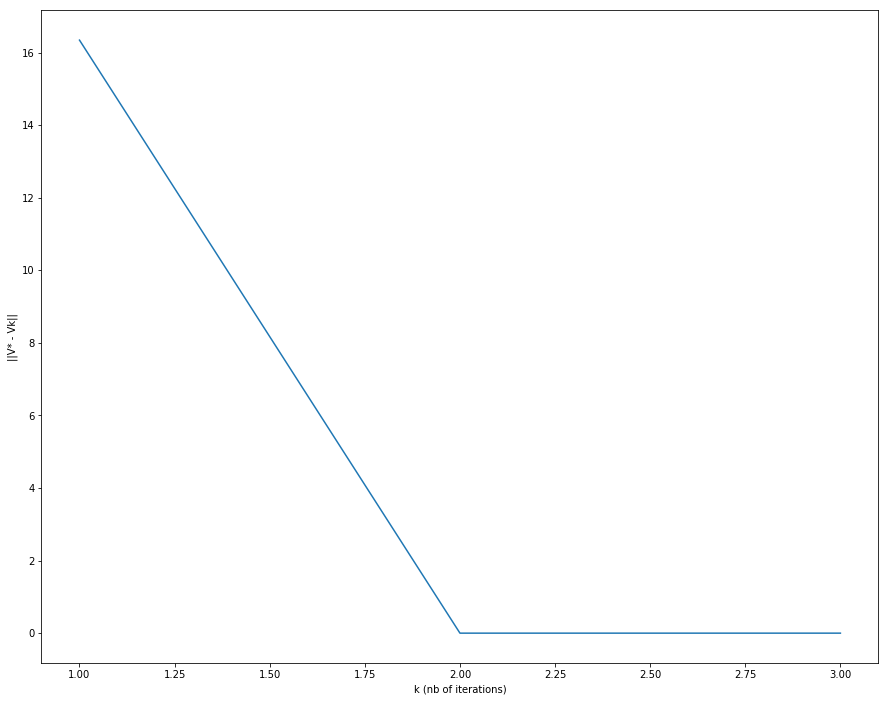
\includegraphics[width=1\linewidth]{images/Q3_PI}
  \caption{Policy Iteration}
  \label{fig:PI}
\end{subfigure}%
\begin{subfigure}{.5\textwidth}
  \centering
  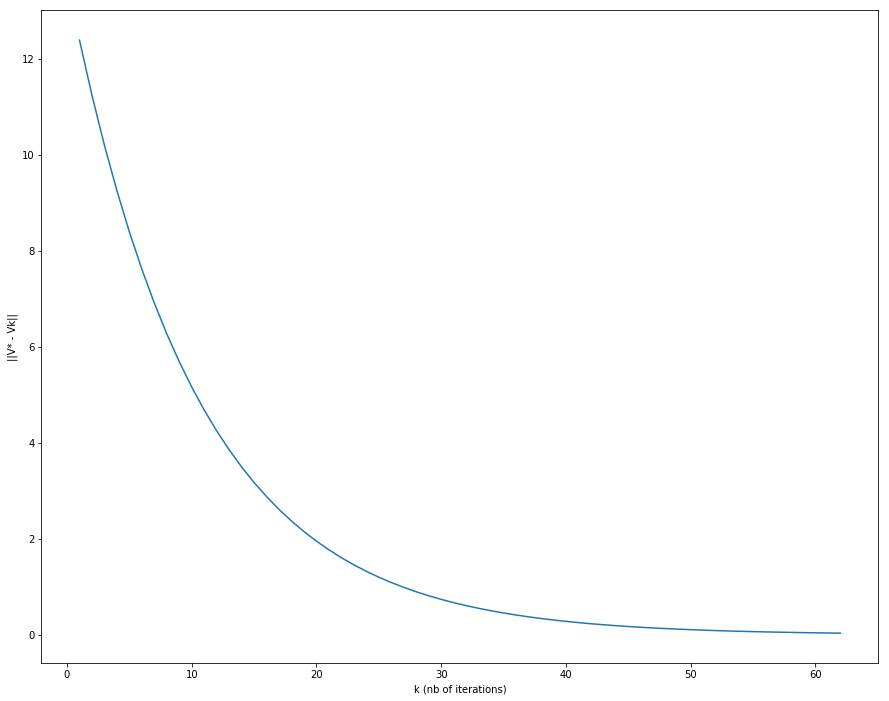
\includegraphics[width=1\linewidth]{images/Q3_VI}
  \caption{Value Iteration}
  \label{fig:VI}
\end{subfigure}
\caption{error rates $||V^{*} - V_k||_{\infty}$ in function of the number of iterations}
\label{fig:error_rate}
\end{figure}

Policy Iteration converges faster than Value iteration. In our experiment, Policy iteration converges in only \textbf{2 iterations} while Value Iteration needed \textbf{60 iterations}. However, each Policy iteration step is much more costlier than Value Iteration as, for each step of Policy Iteration, the algorithm needs to evaluate the current policy.

\section{Reinforcement Learning}
\subsection{A Review of RL Agent/Environment Interaction}
\paragraph{Q4} Let $J_{n} = \sum\limits_{x \in \mathcal{X}} \mu_0(x)V_n(x)$, and $J^{\pi} = \sum\limits_{x \in \mathcal{X}}\mu_0(x)V^{\pi}(x)$ where $\mu_0$ is the uniform distribution, then, using first-visit Monte-Carlo method, we can plot $||J_n - J^{\pi}||$ in function of the number of iterations. Here I choose $E$ (the number of Episode) to be \textbf{1000} and $T_{max}$ the maximum of step in a trajectory to be \textbf{100}. We can see that $J_n - J_{\pi}$ quickly converges towards 0 which is what we want.

\begin{figure}[H]
\centering
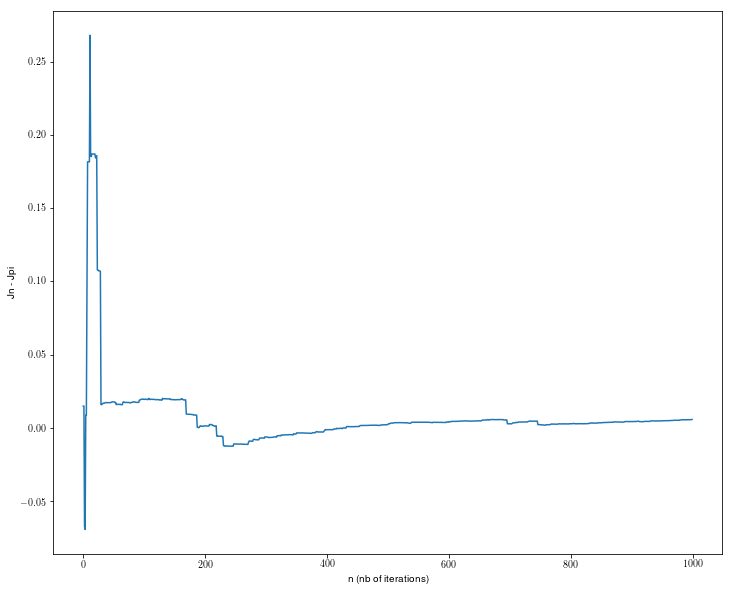
\includegraphics[width=1\linewidth]{images/MC}
\caption{$J_n - J^{\pi}$ in function of the number of iterations using first-visit Monte-Carlo}
\label{fig:MC}
\end{figure}

\paragraph{Q5} I implemented Q-learning algorithm using and $\epsilon$-greedy policy with $\epsilon = 0.1$. I set $E$, the number of episodes to be \textbf{20000}, $T_{max}$, the maximum number of step per trajectory to be \textbf{100}, and I used the learning rate:

$$\alpha_i(x,a) = \frac{1}{N_i(x,a)}$$

where $N_i(x,a)$ is the number of time we visited the state-action pair $(x,a)$ up to iteration $i$. This choice satisfies the Robbins-Monro conditions:

$$\sum\limits_{i} \alpha_i(x,a) = \sum\limits_{i} 1/i = + \infty \quad \text{and} \quad \sum\limits_{i} \alpha_{i}^{2}(x,a) = \frac{\pi^2}{6} < + \infty$$

Figure ~\ref{fig:Q_learning_error_rate} shows the error rates in function of the number of iterations for $\epsilon = 0.1$ and $\epsilon = 0.25$

\begin{figure}[H]
\centering
\begin{subfigure}{.5\textwidth}
  \centering
  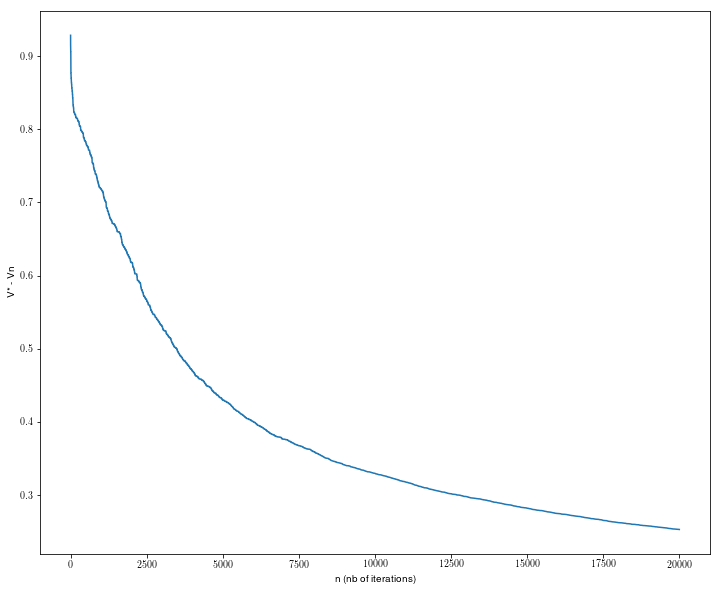
\includegraphics[width=1\linewidth]{images/Ql01}
  \caption{Q-learning with $\epsilon = 0.1$}
  \label{fig:QL10}
\end{subfigure}%
\begin{subfigure}{.5\textwidth}
  \centering
  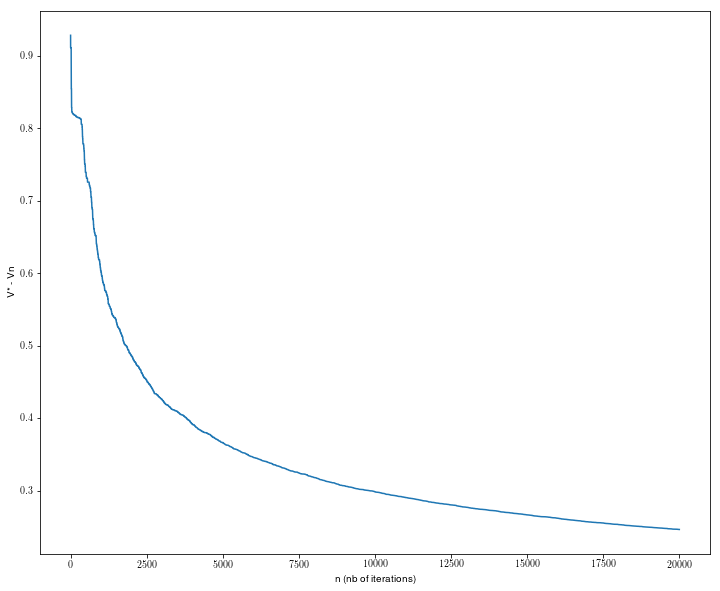
\includegraphics[width=1\linewidth]{images/Ql025}
  \caption{Q-learning with $\epsilon = 0.25$}
  \label{fig:QL25}
\end{subfigure}
\caption{error rates $||V^{*} - V^{\pi_n}||_{\infty}$ in function of the number of iterations}
\label{fig:Q_learning_error_rate}
\end{figure}

Figure ~\ref{fig:Q_learning_R} displays the cumulated reward in function of the number of iterations (Here $E=200$).

\begin{figure}[H]
\centering
\begin{subfigure}{.5\textwidth}
  \centering
  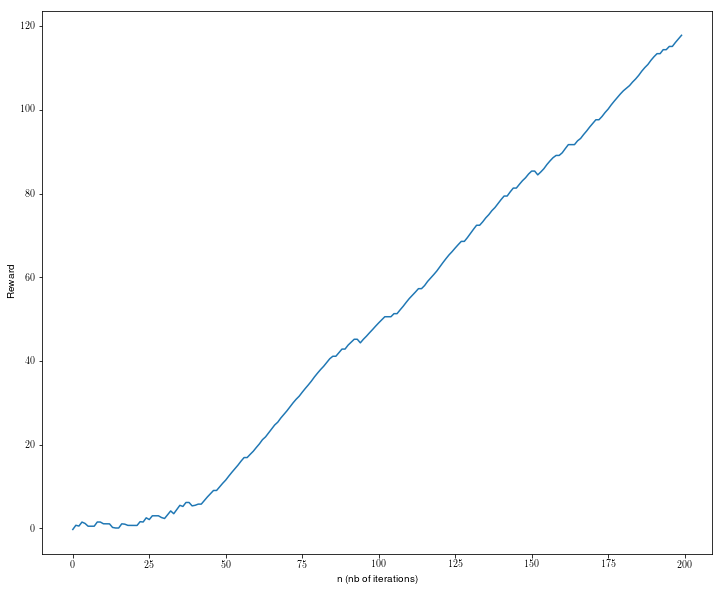
\includegraphics[width=1\linewidth]{images/R10}
  \caption{Q-learning with $\epsilon = 0.1$}
  \label{fig:QL10R}
\end{subfigure}%
\begin{subfigure}{.5\textwidth}
  \centering
  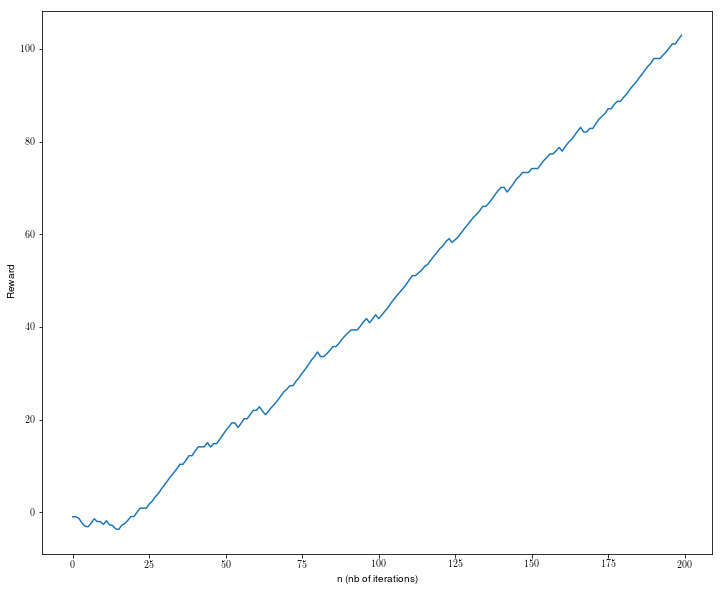
\includegraphics[width=1\linewidth]{images/R25}
  \caption{Q-learning with $\epsilon = 0.25$}
  \label{fig:QL25R}
\end{subfigure}
\caption{Cumulated reward in function of the number of iterations}
\label{fig:Q_learning_R}
\end{figure}

The previous Figures match our intuition. During the first iteration of the algorithm Q-learning doesn't have a very good idea of the optimal policy and so the cumulated reward will oscillate and not increase much. Then after a few iteration the agent have explored most of the state and have a good idea of the action it should do in every step and hence the curve of the cumulated reward will be linear as the agent will most of the time retrieve the same nearly optimal reward. We can also notice that the curve still oscillate a bit. This is due to the epsilon greedy policy. A good idea would be to decay the epsilon with the number of episode. I also added in Table ~\ref{table:Q_learning_table}, the approximated optimal policy computed using Q-learning for different number of iterations. Here I choose $T_{max} = 100$.

\begin{table}[H]
\centering
\begin{tabular}{|l|l|}
\toprule
\textbf{Iterations}  & \multicolumn{1}{c|}{\textbf{Approximated optimal policy}}                  \\ \midrule
$10^2$ & {[}0.645, 0.869, 0.963, 0, 0.276, 0.898, 0, 0.420, 0.678, 0.836, 0.481{]} \\
$10^3$ & {[}0.832, 0.907, 0.982, 0, 0.748, 0.905, 0, 0.660, 0.584, 0.815, 0.430{]} \\
$10^4$ & {[}0.880, 0.930, 0.988, 0, 0.827, 0.921, 0, 0.779, 0.715, 0.847, 0.575{]} \\
$10^5$ & {[}0.876, 0.928, 0.988, 0, 0.817, 0.926, 0, 0.763, 0.805, 0.871, 0.790{]} \\
$10^6$ & {[}0.876, 0.928, 0.988, 0, 0.822, 0.928, 0, 0.775, 0.820, 0.876, 0.823{]} \\ \midrule
$v*$                   & {[}0.877, 0.928, 0.988, 0, 0.824, 0.928, 0, 0.778, 0.824, 0.877, 0.828{]}  \\ \bottomrule
\end{tabular}
\caption{Approximated optimal policy computed for various number of iteration using Q-learning}
\label{table:Q_learning_table}
\end{table}

\paragraph{Q6} The optimal policy of an MDP is not affected by the change of the initial distribution. This is due to the fact that:
\begin{itemize}
\item We explore all the states due to the $\epsilon$-greedy policy
\item the \textbf{optimal action} that should be chosen in a state is independent of the number of times we ended in that state
\end{itemize}

\end{document}
